\documentclass{article}
\usepackage[utf8]{inputenc}
\usepackage{amsmath}
\usepackage{hyperref}
\usepackage{amsthm}
\usepackage{amssymb}
\usepackage[super]{nth}
\usepackage[a4paper, margin=1in]{geometry}
\usepackage{soul,color}
\usepackage{graphicx}
\usepackage{verbatim}
\usepackage{chngcntr}



\title{me srp}
\author{100045495 }
\date{March 2021}

\begin{document}
\begin{titlepage}
    \begin{center}
        \vspace*{1cm}
 
        \textbf{Supervised Dimensionality Reduction Towards \\ 
        Prediction of Phenotype on \\
        Simulated Genotype-Phenotype data}
 
        \vspace{1.5cm}
 
        \textbf{
        Hussain M. Sajwani\\
        100045495@ku.ac.ae\\
        hussainmsajwani@gmail.com
        }
             
        A thesis presented for a Bachelor of Science \\ in Applied Mathematics \& Statistics \\
        Faculty Advisor: Dr. Samuel Feng
        
        \vspace{0.8cm}
        
\includegraphics[width=0.4\textwidth]{university}\\
        Mathematics Department\\
        Khalifa University\\
        May 2021
             
    \end{center}
 \end{titlepage}
\newpage\tableofcontents
\newpage
\begin{comment}
\section{outline}

\begin{enumerate}
    \item intro 
    \begin{itemize}
        \item talk about the bigger genetic problem
        \item disease prediction
        \item genetic data = expensive
        \item genetic data = big ($d \gg n$)
        \item dimensionality reduction and how things break in high dimensions (cite wainright)
    \end{itemize}
    \item lit. review
    \begin{itemize}
        \item related work. recently published bioinfo
        \item related models. stuff in wainright. bigger picture
    \end{itemize}
    \item methodolgy 
    \begin{itemize}
        \item simulation framework. diff parameters and explanation of each
        \item decisions of frame work and methods 
        \begin{itemize}
            \item how PS simulates genotypes if none are provided
            \item how it simulates phenotype
            \item simulation and notation
        \end{itemize}
        \item models to be used and tested
        \begin{itemize}
            \item $p$ threshold
            \item PCA to SVM
            \item Deep $p$ thresholded NN
            \item Vanilla AE 
            \item SAE 
        \end{itemize}
        \item notation
        \item evaluation
        \begin{itemize}
            \item auc
            \item manhattan plot
        \end{itemize}
    \end{itemize}
    \item results
    \begin{itemize}
        \item $p$ thresholding at different parameters of simulation
        \item habiba data high variance 
        \item vanilla AE weights
        \item SAE
        \begin{itemize}
            \item histogram of learnt vs original histogram as $k$ varies and obtain optimal $k=k*$ 
            \item covariance of latent variable. compare it to PCA if possible
            \item weights of first layer $k*$ compare it to manhattan plot of $p$ thresholding
        \end{itemize}
    \end{itemize}
    \item discussion
    \begin{itemize}
        \item optimal k
        \item when does $p$ thresholding fail to give us causal SNPs?
        \item discuss the high variance of models on habiba
        \item compare unsupervised learnt weights vs supervised weights
    \end{itemize}
    \item conclusion
    summer: linkage deq, regulairzatio
\end{enumerate}
\end{comment}
\section{Abstract}
We look at four different methods of dimensionality reduction in the context of utilizing genotype data towards predicting complex traits and disease. Three of which are supervised methods in that they consider a lower-dimensional representation that is more optimal for classification. The methods used are principal components analysis, supervised autoencoder, $p$-value thresholding, and thresholding based on a supervised autoencoder's weights. We benchmark these methods on simulated datasets where ground truth is known \emph{a priori.} This allows us to fully measure the performance of our models. Furthermore, more we train three different classifiers on the lower-dimensional representation obtained from the four dimensionality reduction methods. We compare the AUC of all three methods to rank the performance of each of the dimensionality reduction methods.
\section{Introduction}
Height, weight, IQ, eye color, and many others are all traits of any human being. What determines these traits is a mixture of our genetic information and external factors. Besides controlling traits, genetic information and other external environmental factors can also determine whether someone has a disease or not. A natural question arises: given someone's genetic information, can we estimate the likelihood of them having certain traits or a disease? To answer this we need access to the genetic data of people and the trait of interest. Given how expensive sequencing is and privacy issues, obtaining genetic data is often a hurdle. Even when access to genetic data is obtained, it is often the case that the sample size, $n$, is much smaller than the dimensionality, $d.$ An example we encountered early on, was a dataset provided by Dr. Habiba Al-Safar. The dataset contains BMI information of $n=370$ individuals and $d\approx600,000$ SNPs. Classical statistical methods often fail in this high-dimensional setting \cite{wainright}. Thus if we wanted to use such methods, we will need to find a way of extracting the most important features in our data. To sidestep the expenses and ethical issues of obtaining genetic data, we work entirely on simulated genetic data. In this study, we look at various techniques (supervised autoencoder, weight thresholding, $p$-value thresholding, PCA) and evaluate their performance on simulated genetic data. In particular, we will extract or construct features that we think are more strongly associated with a particular trait. More specifically, in our case, input variables are Single-nucleotide polymorphism (SNPs) which are specific locations (loci) in the human genome that vary in at least 1\% of the population, and we will simulate such genetic data and the associated phenotype.

The genotype of an individual \(i\) is a \(d\)-dimensional vector representing \(d\) SNPs. Let \(x_{ij}\) be a random variable denoting the value of the \(j^{\text{th}}\) SNP of the \(i^{\text{th}}\) individual. Humans are diploid meaning that at each position of DNA, they have two base pairs, one from each parent. The least common base in a population at a particular locus of the DNA is called the minor allele. Each \(x_{ij}\) takes values in \(\{0, 1, 2\}\) representing how much of the minor allele of the \(j^{\text{th}}\) SNP the \(i^{\text{th}}\) individual has. Let \( X \in \mathbb{R}^{n \times d} \) be the matrix containing the \(x_{ij}\)'s mentioned above as its elements. We will call \(X\) the \emph{genotype matrix}. The phenotype is then simulated as some combination of genetic effect (genotype), environmental factors, and observational noise \cite{PS}. The degree to which each of the three components affects the final phenotype can be varied. See below for a discussion on how PS works. The phenotype is an \(n\)-dimensional vector \( y\in\mathbb{R}^n\) where the \(i^{\text{th}}\) entry represents a random variable measuring of some trait.  The constraint of not having enough data typically means we have \(d \gg n\) i.e. we have very few samples compared to how many SNPs we have. This presents a problem as the classical theory of ``large \(n\), fixed \(d\)'' fails to give predictable results. Here, we study tools from modern machine learning which may give answers for how to overcome some of these shortcomings when working with high dimensional data.

\section{Literature review}
This idea of using supervised dimensionality reduction has been studied before. In \cite{montanez}, the authors utilize $p$-values assessing the goodness of a fit of a logistic model between each SNP and polygenic obesity to judge a SNP's effect in predicting polygenic obesity. The authors then pick a threshold $p_0$ and use SNPs with $p < p_0$ to predict polygenic obesity using a deep neural network. Their results claim an AUC (see below for a discussion on what AUC is) of 0.99. Another example is the approach in \cite{alsnet}, where regions of DNA, called promoters, are passed through a convolutional neural network. The promoters with the highest classification accuracy are then passed into a bigger convolutional neural network. Here the authors claim an accuracy of 0.769. The authors in \cite{liu} propose a novel method of training neural networks in high dimensional regimes. Using some insight from functional analysis, they propose a way of regularizing the weights with the $l_p$ norm by looking at the $l_q$ norm, with $\frac{1}{p} + \frac{1}{q} = 1$ of the neural network's gradients. When this regularization is applied, the authors claim an AUC of 0.926 on a dataset with $n=85$ and $d=22,283.$
\section{Methodology}
To have a good understanding of how models behave, we need to test them out in various settings and scenarios. Testing our models on real data is expensive and time-consuming given how hard it is to get genetic data. We also need ground truth (a priori knowledge) to test our models on. This is why we look at simulated genetic data.
\subsection{PhenotypeSimulator}
We will use the \texttt{PhenotypeSimulator} (PS) R package \cite{PS} to simulate genotype-phenotype relations. PS can either take the genotype as input or simulate its own relatively simple genotype. Since we do not have access to data, we decided to go with the option of simulating the genotypes using PS. The simulated genotypes are very simple. The genotype matrix $X$ is simulated as 
\[ 
\mathrm{vec(X)} \sim \mathrm{Bin}(nd, U).
\]
Where $U$ is uniformly distributed over $\{(p_0, p_1, p_2\}.$ Where each $p_k$ represents the allele frequency. e.g. $p_0$ is the frequency of there being 0 of the minor allele. The phenotype is simulated to be the output of the genotype and some external factors. We use the default values provided by \texttt{PhenotypeSimulator} of $(0.4, 0.2, 0.1).$ Mathematically speaking, the phenotype is some convex combination of genetic factors and external factors. In this study, we constrain ourselves to only looking at the genetic factors. In all simulations, we let external factors only contribute 5\% to the simulated phenotype. The genotype contribution is further broken down into two components. The first controls how much a select group of SNPs contributes to the phenotype. This select group of SNPs is called causal SNPs. Typically, this is a very small amount of SNPs. We will call the number of causal SNPs $d_c$ and their effect on the final phenotype $h_2^s.$ The $s$ in $h_2^s$ stands for causal SNPs and the 2 is to indicate that we are simulating a bi-allelic (diploid) genotype. The second component controls how much the background polygenic effect of all SNPs on the final phenotype. This is different from the first component in that there are no select few SNPs that control the phenotype but rather all SNPs contribute. This second component will be called $h_2^b.$ Both components are nonnegative real numbers such that $h_2^s + h_2^b = 1.$ We will denote each simulated dataset by a with 4-tuple 
\[
(n, d, d_c, h_2^s).    
\]
These will represent the parameters of interest to us in PS. The phenotype generated is then some vector $\hat{y} \in \mathbb{R}^n$ which we convert into a binary vector $y \in \{0, 1\}^n$ by thresholding $\hat{y}$. An example of this is BMI and obesity. If we are trying to study obesity, we do not care about the particular value of BMI. We just care if it is above or below some threshold. See figure \ref{fig:phenotypesimulator} for a summary of how PS works.

\begin{figure}
    \centering
    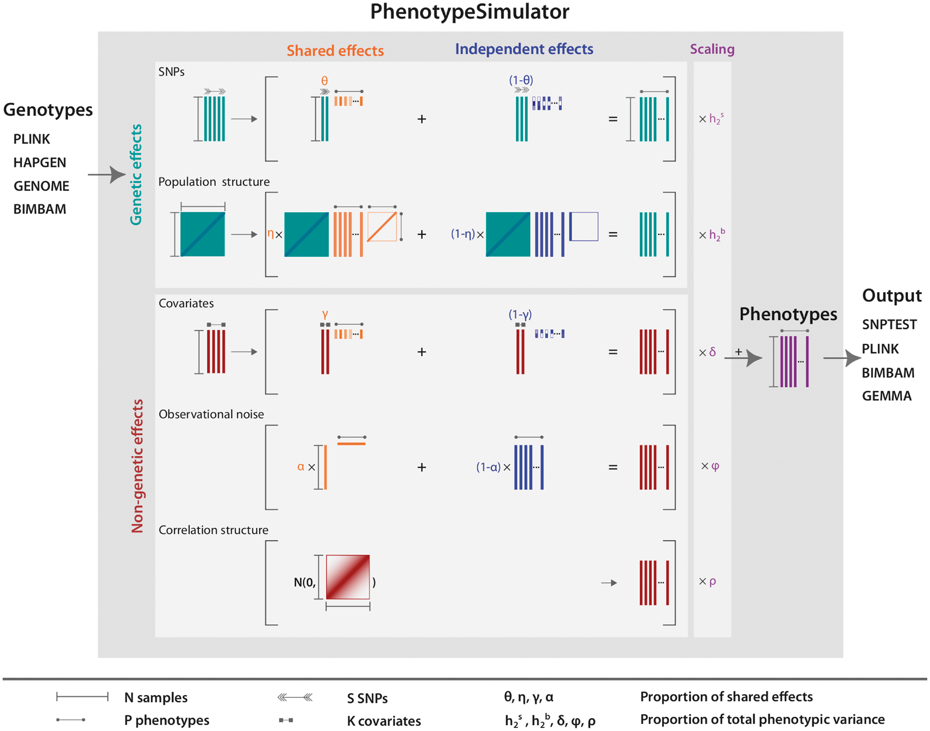
\includegraphics[width=0.5\textwidth]{pheno.png}
    \caption{A brief summary of how \texttt{PhenotypeSimulator} works. The top teal part is the genetic component of the simulation accounting for 95\% of phenotype in our simulations. The bottom red part is the nongenetic 5\% component. Figure is from \cite{PS}.}
    \label{fig:phenotypesimulator}
\end{figure}

\subsection{Dimensionality reduction methods}
In this study, four dimensionality reduction algorithms will be tested. The first two algorithms will simply extract $k$ features the algorithm thinks are relevant and discard the rest. The other two will extract $k$ new features built from the original $d$ features. 
\subsubsection{Neural networks, autoencoders, and supervised autoencoders}
A typical binary classifier deep neural network, $\mathrm{DNN}:\mathbb{R}^d \longrightarrow [0, 1]$, is a model made of a sequence of affine transformations that are passed, elementwise, through some nonlinearties. Let $\{d^{(1)},\dots,d^{(L)}\}\subset \mathbb N$ be a sequence of positive integers. Given an observation $x \in \mathbb R^d,$ a DNN apply some affine transformation represented by a matrix $W^{(1)} \in \mathbb R ^ {(d^{(2)} + 1) \times (d+1)}$, called the weight matrix, (the +1 is added to represent the bias term of the affine model so that every observation $x$ is padded with a constant variable to reflect this bias) and then pass it elementwise into some nonlinear function, called the activation function, $g^{(1)}$. This process is repeated $L$ times with the $l^{\text{th}}$ time represented with an affine transformation with matrix $W^{(l)} \in \mathbb{R}^{(d^{(l)} + 1) \times (d^{(l-1)} + 1)}$ and a nonlinear function $g^{(l)}.$ The $l^{\text{th}}$ repetition is called the $l^{\text{th}}$ layer of the neural network. $d^{(l)}$ is called the width of the $l^{\text{th}}$ layer and the elements of $W^{(l)}$ are called the weights of the layer. The final layer, the $L^{\text{th}}$, has output size $d^{(L)}=2$.The output here can be interpreted as two probabilites of the sample having $y=0$ or $y=1$, respectively. Common choices of $g^{(l)}$ are 
\[
\mathrm{ReLU}(x) = \max\{0, x\}.    
\]
and 
\[
    \sigma(x) = (1+e^{-x})^{-1}.
\]
For a graphical interpretation of a neural network look at figure \ref{fig:nn}.
\begin{figure}[t]
    \centering
    \includegraphics[width=0.5\textwidth]{imgs/neural_net2.jpeg}
    \caption{A graphical representation of a neural network. Each colored box represents a layer. The connections (black arrows) between the layers are the weights $W^{(l)}.$ This image was downloaded from: \url{https://cs231n.github.io/neural-networks-1/.}}
    \label{fig:nn}
\end{figure}
The choice of $L$, $d^{(l)}$, and $g^{(l)}$ for any $l=1,\dots,L$ is made by the designer of a neural network. These parameters which are to up to the designer are called the hyperparameters of the neural network. The choice of $W^{(l)}$ for all $l = 1,...,L$ though is determined by an optimization algorithm. For a set of weight matrices $W=(W^{(1)},\dots,W^{(L)})$ we evaluate the performance of the neural network by comparing its prediction $\hat{y} = \mathrm{DNN}(x;W)$ with the actual value of $y.$ Remember that $\hat{y}$ is a two dimensional vector. Its second element $\hat{y_1}$ is the probability the neural network "thinks" that $y=1.$ In this study we use cross-entropy \cite{dlbook} as our objective function to evaluate the performance of a DNN. Cross-entropy is defined as 
\begin{align*}
    J(W)
    &= -\mathbb{E}_{x,y \sim p_{\text{observed}}}\log \mathrm{DNN}(x;W)_1 \\
    &= -\log \hat{y}.
\end{align*}
The goal now will be to find $W$ such that $J(W)$ is minimized. First, we initialize all the weights of all of the neural network randomly. Then we pass an observation $x$ through the network and observe some $\hat{y}.$ With this, we can evaluate $J(W)$ to compare $y$ and $\hat{y}.$ We can use this information to judge how good the weights $W$ are. The weights are then updated to reflect the information just attained. This process is repeated iteratively until a minimum is reached. We use the Adam optimizer \cite{adam} to find the optimal weights $W.$ The parameters used are $\alpha=0.001$,  $\beta_1=0.9$, $\beta_2=0.999$, and $\epsilon=10^{-7}.$

A logistic regression model can be modeled as a one-layer neural network with $g^{(1)}(x) = (1+e^{-x})^{-1}.$ and $W \in \mathbb{R}^{2 \times (d + 1)}$.

\begin{figure}[t]
    \centering
    \includegraphics[width=0.5\textwidth]{imgs/ae.jpeg}
    \caption{An example of an autoencoder with two layers in the encoder and decoder parts. The red units are the bottleneck. This image was downloaded from \url{https://www.compthree.com/blog/autoencoder/}}
    \label{fig:ae}
\end{figure}

Autoencoders are a special type of deep neural network where the final layer is not some binary variable but rather a $d$-dimensional vector. Figure \ref{fig:ae} shows a graphical depiction of an autoencoder. Given an input to the neural network $x \in \mathbb{R}^d,$ the goal of an autoencoder is to first encode $x$ into some smaller vector $x_k \in \mathbb{R}^k$ with $k < d$ and then using $x_k$ to reproduce, to its best ability, the input vector $x$. Then let the first $\lfloor L/2 \rfloor$ layers have widths $d^{(1)} > d^{(2)} >...> d^{(\lfloor L/2 \rfloor)}$ with $k := d^{(\lfloor L/2 \rfloor)}.$ This part of the autoencoder is called the encoder. The other layers are to be mirrored around the middle layer. i.e. $d^{(1)} = d^{(L)}, \, d^{(2)} = d^{(L-1)},\dots,$ and so on. This does not mean these layers have the same weights. We are only imposing that the widths of the layers be tied together. Inspired by PCA, there has been some work in the literature exploring weight-tied autoencoders. See \cite{tied} for a discussion on the matter. This part of the autoencoder is called the decoder. The middle layer of the autoencoder will be called the latent space. The final layer then produces a $d$-dimensional vector $\hat{x}$ which we interpret as the reconstruction of $x.$ To fit an autoencoder, we use MSE as the objective function to be minimized as cross-entropy is not valid. For a vector $x$ that is approximated with $\hat{x}$ by the autoencoder, MSE is defined as $\mathrm{MSE}(W) = (x-\hat{x})^2.$ We use Adam \cite{adam} to optimize this as well. The encoded representation then comes from taking the output of the middle layer. Notice that these features are extracted features; they might not have a biological interpretation. This is one downside to dimensionality reduction methods that extract features rather than select them. Also, notice that nowhere in the above description do we use the information from the phenotype $y.$ We are simply looking at a lower-dimensional representation of the genotype without taking into account the response of the phenotype. This could be an issue as the autoencoder might not learn to emphasize the presence of a causal SNP. For this reason, we use supervised autoencoders.

We combine the two tasks of classification and reconstruction into a neural network structure called supervised autoencoders \cite{sae}. Let
\begin{align*}
    \mathrm{enc}&:\mathbb{R}^d \longrightarrow \mathbb{R}^k \\
    \mathrm{dec}&:\mathbb{R}^k \longrightarrow \mathbb{R}^d \\
    \mathrm{clf}&:\mathbb{R}^k \longrightarrow [0, 1]. 
\end{align*}
These functions represent the encoder part of an autoencoder, the decoder part, and a classifier that takes in a $k$ dimensional representation of a $d$-dimensional vector. Assume that all of these functions are parts of a neural network (each represents a sequence of affine transformations passed through some nonlinear functions.) An autoencoder, $\mathrm{AE}$ is then formed by composition
\[
AE = \mathrm{dec} \circ \mathrm{enc}.    
\]
And the supervised part, $S$, of a supervised autoencoder is formed as 
\[
S = \mathrm{clf} \circ \mathrm{enc}.
\] 
We train both of these two parts concurrently. The objective function that we use will be some convex combination of the two previously defined objective functions. As always let $W$ and let $\rho \in [0, 1]$ be the weights of the supervised neural network autoencoder (all three parts of it) then the objective function is defined as 
\[
J(W) = \rho J_{\mathrm{AE}}(W) + (1-\rho) J_{S}(W).
\]
Where $J_{AE}$ is the objective function of reconstruction and $J_{S}$ is the objective function of the classifier. We will call the variable $\rho$ the reconstruction weight. It determines how much emphasis the learning algorithm should put on the reconstruction objective. $1-\rho$ is the classification weight. It determines the emphasis on the classification objective. This approach to learning is called multitask learning. 

As is the case with a classifier deep neural network, the choice of depth and widths is up to the designer to determine. Here we also add the choice of what classifier to use. We look at various choices for these hyperparameters. Unless stated otherwise, assume that $\mathrm{clf}$ is a logistic regression model.

\subsubsection{Principal components analysis (PCA)}
Principal components analysis (PCA) is the second dimensionality reduction method we consider that considers complex features as its extracted features. PCA works by finding a set of the orthogonal basis for $\mathbb{R}^d$ such that the variance of the data along each of the basis vectors is maximized. One can think of this as taking a straight line parallel to one of the orthogonal vectors and projecting all of the datasets on it. The variance we try to maximize is the variance of the projected dataset onto the straight line. The theory here is that more variance implies more interesting information. The basis vectors are then sorted by how much variance the dataset has in a vector's direction and we take the top $k$ vectors. Finally, we project the data onto the linear subspace formed by the top $k$ vectors. The projected data is the reduced representation of the original dataset $X.$

The set of orthogonal basis is found by studying the covariance matrix of $X$, 
\[
    \frac{1}{n}XX^{T}
\] 
(without loss of generality, assume the variables have mean zero.) Note that this representation of the covariance matrix is made with respect to the canonical basis of $\mathbb{R}^d.$ To maximize variance means to maximize the diagonal of the covariance matrix. This means that we need to diagonalize the matrix to find our sought-after representation. This can be done since covariance matrices are, by definition, symmetric and hence are always diagonalizable and have orthogonal eigenvectors. Finally, the basis we want is the set of eigenvectors of the covariance matrix.

It can be shown that training a two layers autoencoder with linear activation on both layers (i.e. $g^{(1)}(x) = g^{(2)}(x) = x$) and $d^{(2)} = k$ is equivalent to finding the subspace spanned by the top $k$eigenvectors found above \cite{aepca}.
\subsubsection{p-value thresholding}
We will look at two thresholding methods. The first one is called $p$-value thresholding. It is a commonly used method in the field of bioinformatics to determine the strength of the association between a certain SNP and a certain phenotype. This method identifies associations between SNPs and a phenotype by fitting $d$ logistic regression models between each of the $d$ SNPs and the phenotype $y.$ Then a $p$-value is calculated to measure the strength of the association. That $p$-value is then used to quantify the strength of the association between a particular SNP and the phenotype. Then we select $k$ SNPs with the $k$ highest value of $-\log_{10}p.$ This is called thresholding because typically, one would select some value of $p_0 \in (0,1)$, called the threshold, and simply select all SNPs with $p$-values such that $-\log_{10}p \geq -\log_{10}p_0.$ When selecting such a threshold one has to be aware of issues concerning multiple hypothesis testing and adjust $p_0$ accordingly \cite{bonferroni}. The work of Amina Salem from last year deals with this issue and how to correct it when testing for associations. However, since we are interested in comparing this method to other methods, we choose a top-$k$ approach.
\subsubsection{AE weight thresholding}
Inspired by $p$-value thresholding, we propose a new method of thresholding based on the learnt weights of an SAE. Another approach we use to select features is based on the autoencoder. After training a supervised autoencoder, we look at the weights of the first layer $W^{(1)} \in \mathbb R ^ {(d^{(2)} + 1) \times (d+1)}$ and form a vector,
\[
a = \sum_{j=1}^{d^{(2)} + 1} \left(W^{(1)}_{;j}\right)^2  
\]
for the $i^{\text{th}}$ SNP. The idea here is that if a SNP is highly associated with the phenotype, then its weights on the first layer should be higher in magnitude. In other words, $a_i$ should be higher for more relevant SNPs. Irrelevant SNPs receive the opposite treatment where their weights get closer to 0. From this, we pick the top $k$ SNPs corresponding to the highest $k$ values of $a.$

\subsection{Evaluation} \label{method_eval}
Since our overarching goal is to predict a phenotype, we will use the performance of classifiers on reduced data to measure the efficacy of our reduction techniques in extracting relevant features. We will use three different classifiers: a support vector machine \cite{islr} with a radial basis function kernel, a logistic regression model, and a deep neural network. Unless stated otherwise, we always break down each dataset into a 0.6/0.2/0.2 training, validation, and testing split. This means models only train on $0.6n$ of the simulated datasets.   

The architecture of the DNN used is inspired by the architecture used by \cite{montanez}. It is 7 layers deep including the input and output layers. The input layer has width $d^{(1)}=k$ (the size of reduced dimensionality.) The rest of the layers are of width 50, 50, 40, 30, 20, 2. To reduce overfitting, we use dropout on the second and third layers. Dropout randomly selects a proportion of the entries of the vector and sets them equal to zero during training \cite{dropout}. The proportion in this study is 0.5. We also use $l_1$ and $l_2$ regularization on all layers. The parameters used for all layers are $3 \times 10^{-6}$, and $6.5 \times 10^{-5}.$
 
\subsubsection{Area under the curve (AUC)}
\begin{figure}[t]
    \centering
    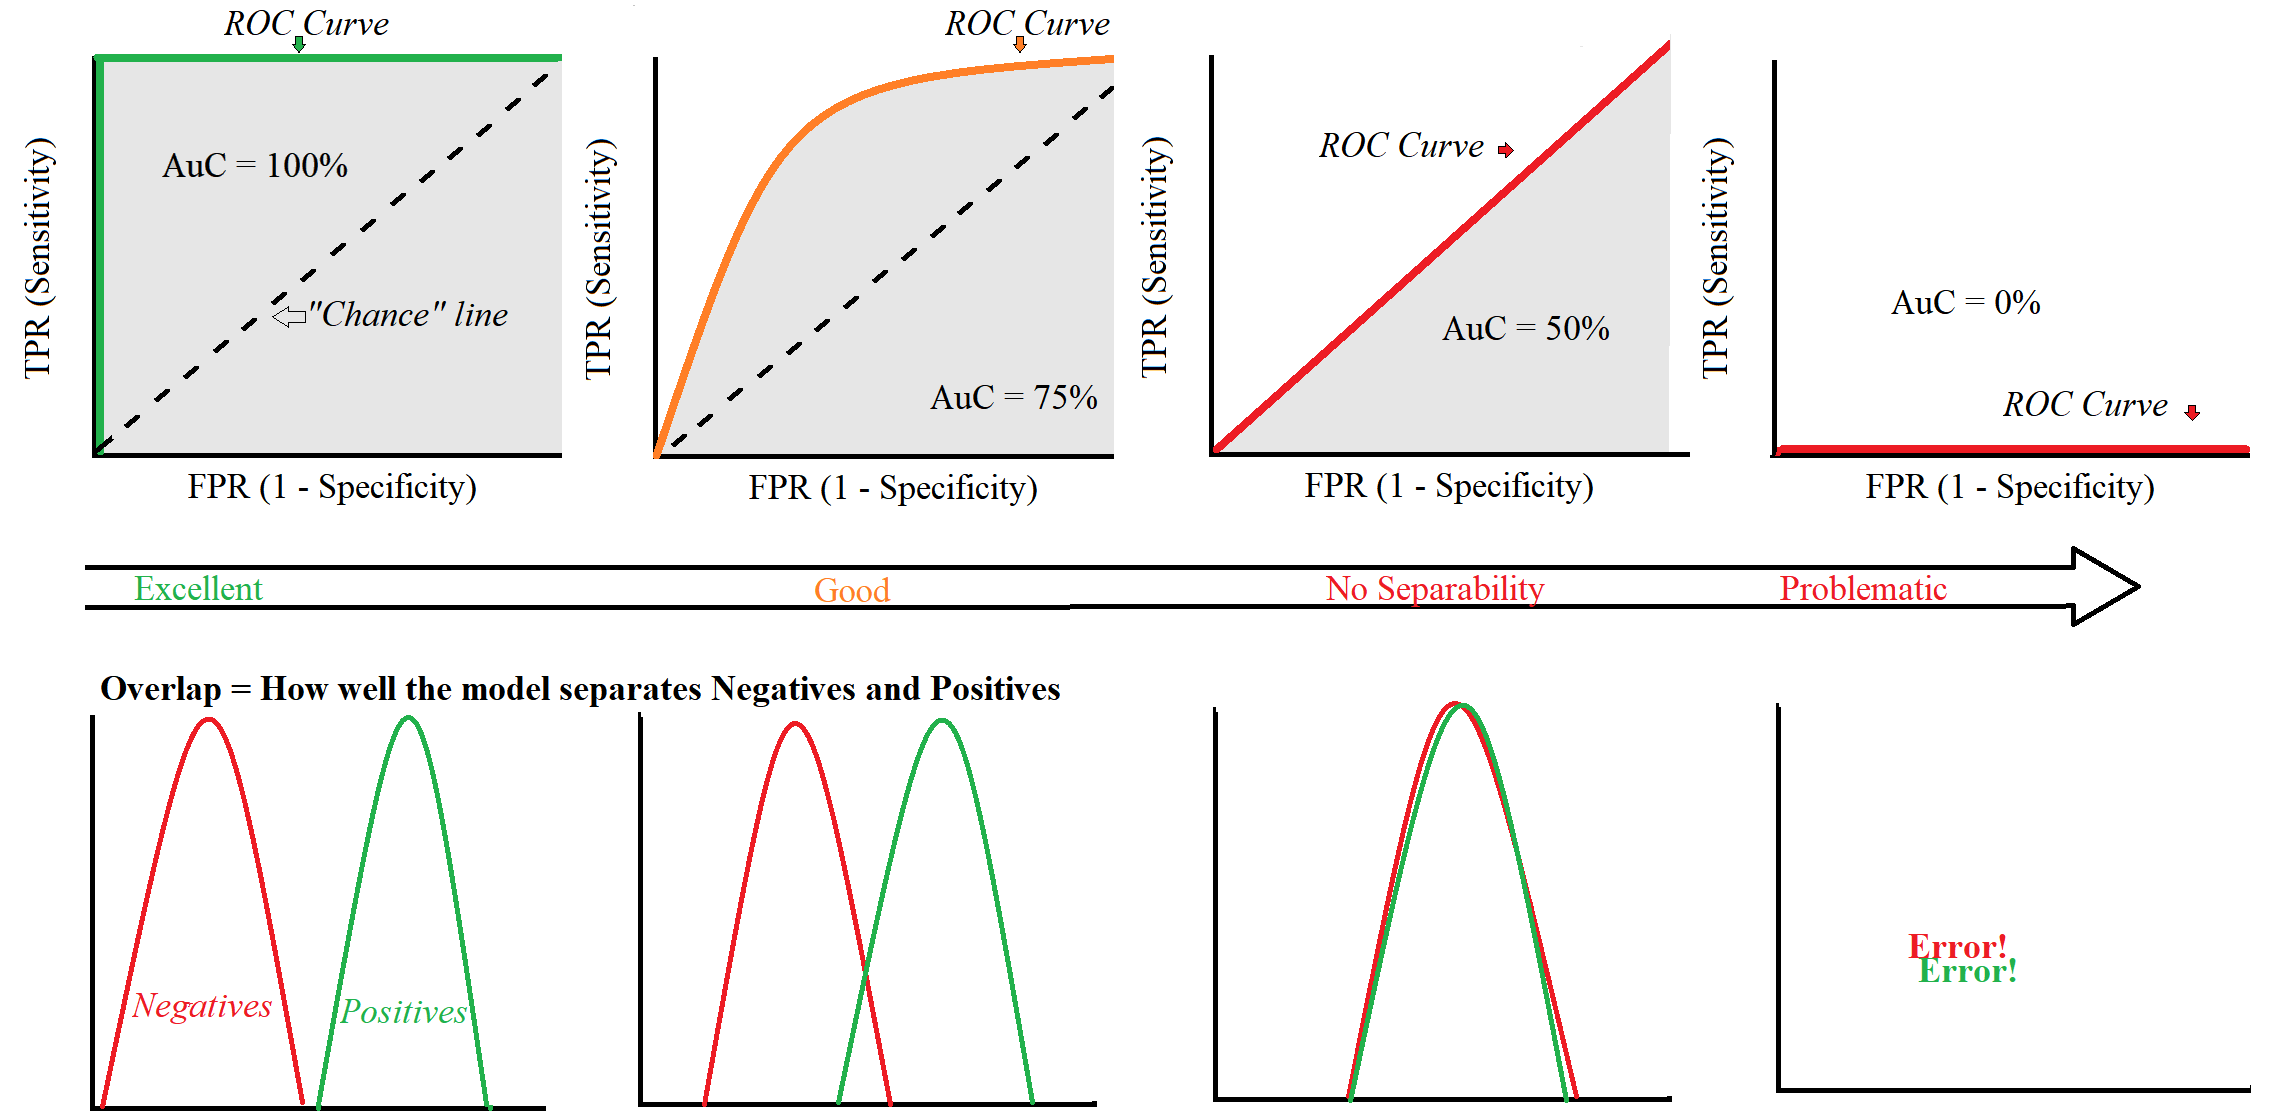
\includegraphics[width=0.8\textwidth]{imgs/roc.png}
    \caption{Demonstration of ROC curves. The leftmost panel represents the perfect scenario for a classifier in which it has learnt a perfect separation to the observation based on their class. Given an observation, a classifier with AUC=100\% is able to always predict which class the observation belongs to. The second panel shows a more attainable ROC curve. The third panel shows a case where the classifier has not learnt anything and leaves classification up to chance. The last panel shows a ROC curve of a model that does worse than chance. It will always give the wrong label. The picture was downloaded from \url{https://www.datasciencecentral.com/profiles/blogs/roc-curve-explained-in-one-picture}}
    \label{fig:roc}
\end{figure}
To measure the performance of the classifiers, we will use a metric called area under the curve (AUC.) The curve in question here is the receiver operating characteristic curve (ROC.) The ROC curve can be thought of as a parametric curve with respect to a thresholding parameter $t \in [0, 1].$ The three methods we test output a number which we interpret as a probability of an observation falling into one of two classes. For any binary classification task, we set some threshold $t$ on the probabilities by which we determine what to label an observation. For certain cases, we require very high certainty so we only label an observation if our models give it a very high probability of being that label so we set a relatively high threshold $t$. For any choice of threshold, we calculate two parameters. The true positive rate $\mathrm{TPR}(t)$ and the false positive rate $\mathrm{FPR}(t)$. Given a labeled dataset, $\mathrm{TPR}(t)$ determines what proportion of observations with a positive label ($y=1$ in our case) were assigned to have a positive label by the model under consideration and a threshold $t.$ The $\mathrm{FPR}(t)$ is the proportion of observations with a negative label ($y = 0$ in our case) were assigned to have a positive label by the model and a threshold $t.$ The ROC curve then is given by 
\[
    \{(\mathrm{FPR}(t), \mathrm{TPR}(t)) \, |\, t\in[0,1]\}.
\]
A perfect classifier will assign all positive observations a positive label and not assign any negative observations a positive label. This means that the ROC curve will hug the top left corner of the unit square. If we choose our classifier in such a way that it labels each observation based on the flip of a fair coin, then the ROC curve will be the diagonal line TPR = FPR. See figure \ref{fig:roc} for an illustration. This motivates the definition of AUC. Finally, the AUC is defined to be the area under the curve of the ROC curve and above the FPR axis. For a perfect classifier where the curve hugs the top left corner of the unit square, the area under the curve is 1. The fair coin classifier will have AUC 0.5. We will use AUC to measure the performance of the classifiers.

\subsubsection{Precision and Recall}
To understand how well our thresholding is doing, we will use two quantities called precision and recall that give us an idea of how well our thresholding is separating causal SNPs from non-causal ones. Precision and recall are typically used to assess classifiers. We treat thresholding as a classifier that assigns a positive label to quantities above (or below) the threshold and negative labels to quantities below (or above) the threshold. As was the case with the true positive rate and the false positive rate, precision and recall are functions of the thresholding parameter $t.$ Precision is defined as 
\[
    \mathrm{Prec}(t) = \frac{\mathrm{TPR}(t)}{\mathrm{TPR}(t) + \mathrm{FPR}(t)}.
\]
It is interpreted as the proportion of all observations that have been assigned a positive label that is positive. Recall is defined as 
\[
    \mathrm{Rec}(t) = \frac{\mathrm{TPR}(t)}{\mathrm{TPR}(t) + \mathrm{FNR}(t)}.
\]
Where $\mathrm{FNR}(t)$ is the rate of positive observations that are assigned a negative label. Recall is interpreted as the proportion of all positive observations that have been labeled correctly. 
\section{Results}
Computations were carried on a Linux machine running Ubuntu 18.04.5 with 64GB RAM, 2 Nvidia Tesla K20c GPUs, and 12 Xeon E5-2603 cores. Miniconda3 Python 3.7.9 is used for all computations. Neural network based models have been impelmented in \texttt{TensorFlow} 2.2.0 \cite{tf}. Other models used have been implemented using \texttt{scikit-learn} 0.23.2 \cite{scikit-learn}.
\subsection{Architecture of autoencoder}
\begin{figure}[t]
    \centering
    \begin{minipage}{.5\textwidth}
        \centering
        \includegraphics[width=1\linewidth]{imgs/multiple_histogram.jpeg}
    \end{minipage}%
    \begin{minipage}{.5\textwidth}
        \centering
        \includegraphics[width=1.2\linewidth]{imgs/wasser.jpeg}
    \end{minipage}
    \caption{\emph{Left:} Each panel has a histogram of the original genotype matrix $X$ and a histogram of $\hat{X}$, the autoencoder's attempt at reconstructing $X.$ The genotype is simulated with parameters $(600, 1000, 10, 0.5)$. The autoencoder is two layers deep with $\rho=0.8$ with $k \in \{5, 10, 20, 50, 100, 250, 500, 750, 1000\}$ \emph{Right: }Wasserstein distance from original histogram to reconstructed ones from autoencoders with size $k$.}
    \label{fig:bottlenecking}
\end{figure}
On the left of figure \ref{fig:bottlenecking} we see a histogram of how much each possible occurrence of the minor allele is present at any SNP. We see that most loci (location on DNA) have 0 occurrences of the minor allele. Fewer loci have 1 occurrence, and even fewer loci have 2 occurrences. We simulate a dataset with parameters $(600, 1000, 10, 0.5)$ and train 9 supervised autoencoders with $\rho = 0.8$ and values of $k$ ranging from 1000 and 5. It can be seen from the histograms that as $k$ decreases (i.e. the bottleneck tightens), the autoencoder learns to just focus on reconstructing as many zeros as possible. 

To quantify the observed effect, we utilize the Wasserstein distance \cite{wasserstein}. The Wasserstein distance is a way of measuring distances between two probability distributions. It can be shown that the Wasserstein measure defines a metric on the set of all Borel measures on some metric space. This allows us to measure the distance between the original histogram of the dataset and the autoencoder's attempt at reconstructing it. The rightmost panel of figure \ref{fig:bottlenecking} shows the Wasserstein distance between the original histogram and the reconstruction. This confirms what we see in the middle panel. As the bottleneck size $k$ decreases, the reconstruction becomes harder to learn.

To further understand the learnt supervised autoencoder (SAE) we look at the extracted features. Specifically, we look at the covariances of the extracted features and how that covariance varies with $k$ and $\rho.$ For this, we train a few ReLU activated SAEs with $\rho \in \{0.2, 0.6, 1\}$ and different $k$ values on a dataset. The results shown in figure \ref{fig:cov} show the correlation matrices of the extracted features. It can be seen that as $\rho$ approaches 1 i.e. the SAE approaches an AE, the correlation matrix tends to become more diagonal. If the SAE has learnt to extract a constant feature, then the variance of that feature will be zero and hence correlation will be undefined. When this happens we let the correlation be 0.

\begin{figure}[t]
    \centering
    \begin{minipage}{.333\textwidth}
        \centering
        \includegraphics[width=1\linewidth]{imgs/cov_rw0.2.jpeg}
    \end{minipage}%
    \begin{minipage}{.333\textwidth}
        \centering
        \includegraphics[width=1\linewidth]{imgs/cov_rw0.6.jpeg}
    \end{minipage}%
    \begin{minipage}{.333\textwidth}
        \centering
        \includegraphics[width=1\linewidth]{imgs/cov_rw1.jpeg}
    \end{minipage}
    \caption{Correlation matrices of extracted features of ReLU activated SAE. Each panel represents the results of a SAE trained with $\rho=0.2, 0.6, $ and $1$, respectively. Each panel contains nine subpanels which show the correlation matrices for values of $k \in \{5, 10, 20, 50, 100, 250, 500, 750, 1000\}.$ The leftmost, $\rho=1$, panel confirms theory that an AE will learn a diagonal correlation matrix, like PCA. The other two SAE with $\rho \neq 1$ do not learn uncorrelated features. Note that if an entry on the diagonal is zero, then the SAE learnt a constant feature.}
    \label{fig:cov}
\end{figure}

\begin{figure}[t]
    \centering
    \begin{minipage}{.5\linewidth}
        \centering
        \includegraphics[width=\textwidth]{imgs/p_manhattan.jpeg}
    \end{minipage}%
    \begin{minipage}{.5\linewidth}
        \centering
        \includegraphics[width=\textwidth]{imgs/ae_manhattan.jpeg}        
    \end{minipage}
    \caption{Example thresholding on a single dataset with $h_2^s = 0.75$ and both thresholding methods. }
    \label{fig:manhattan}
\end{figure}

\begin{figure}[t]
    \centering
    \includegraphics[width=0.7\textwidth]{imgs/prec_rec.jpeg}
    \caption{Violin plots of precision and recall of both thresholding methods over all 25 datasets for each value of $h_2^s$ and $k$. In both precision plots, precision goes up as $h_2^s$ increases and goes down as $k$ increases. Recall increase with both $k$ and $h_2^s$. \emph{Top left}: precision of $p$ value thresholding. In all circumstances, $p$ thresholding has zero variance. \emph{Top right:} recall of $p$ thresholding. This also has zero variance. \emph{Bottom left}: precision of AE weights thresholding. High variance for lower values of $k$ and decreases with $h_2^s.$ \emph{Bottom right:} Recall of AE thresholding. Low variance on lower values of $k.$ }
    \label{fig:prec_rec}
\end{figure}

\subsection{Thresholding} \label{results_th}
To compare the two thresholding methods we look at how well they capture causal SNPs in various settings of $h_2^s.$ To do this we utilize the precision and recall quantities defined above. We simulate 125 datasets with parameters $(600, 1000, 10, h_2^s)$ for $h_2^s \in \{0.05, 0.25, 0.5, 0.75, 1\}$ and perform both types of thresholding on each of the 25 datasets. The SAE used has $k=300$ and $\rho=0.3.$ The $k$ used for thresholding is taken to be $k \in \{5, 25, 100, 300\}.$ Figure \ref{fig:manhattan} shows an example of manhattan plots where the $x$ axis is all of the SNPs and the $y$ represents how strongly associated the SNP is to the phenotype. Figure \ref{fig:prec_rec} shows violin plots of precision and recall overall 25 datasets for each value of $h_2^s$. The straight lines mean that there was no variance in the quantity being measured. We can see that $p$-value thresholding better variance than AE thresholding and overall is better in terms of AUC. 

\subsection{Classification}
In the following sections, we use the same 125 simulated datasets from the thresholding section.
\begin{figure}[t]
    \centering
    \includegraphics[width=1\textwidth]{imgs/pca.jpeg}
    \caption{Classification results of three models trained after reducing dimensionality using PCA. In all three models, PCA has done a bad job of extracting information that is useful for classification. The AUC barely goes above 0.8 in some cases. }
    \label{fig:pca_auc}
\end{figure}
Here we benchmark the dimensionality reduction methods on classifiers. We use the same 125 simulated datasets in section \ref{results_th} and apply the four reduction methods discussed. We reduce the dataset to $k$ features with $k \in \{5, 25, 100, 300\}$. Then we train three classifier models on each of the reduced representations for every $k.$ The classifier models to be used are the same ones mentioned in \ref{method_eval}
\subsubsection{Classification with PCA reduced dataset}
Figure \ref{fig:pca_auc} shows the classification results of the three models trained on the projected dataset with different values of $h_2^s$. The SVM and logistic model seem to outperform the deep neural network. The AUC does not exceed 0.9 in all of the models. With respect to each model, the performance of the model does not change with $h_2^s.$ Increasing the value of $k$ improves performance. 
\subsubsection{Classification with SAE reduced dataset}
\begin{figure}[t]
    \centering
    \includegraphics[width=\textwidth]{imgs/learnt.jpeg}
    \caption{Classification results of three models trained after reducing dimensionality using SAE with $\rho=0.3$. All methods seem to be doing better than PCA. \emph{Top left:} the performance of the supervised part of the supervised autoencoder. \emph{Top right:} results of an SVM trained on the latent space of the autoencoder}
    \label{fig:sae_auc}
\end{figure}
Figure \ref{fig:sae_auc} shows the results of passing through the representation an SAE learns in its middle layer to a classification algorithm. SAE seems to be more sensitive to $h_2^s$ than PCA. Each color, on average rises up as $h_2^s$ is increased. Furthermore, in lower $k$'s, SAE's results seem to outperform PCA's. Even though the supervised branch of the SAE is made of a logistic regression model, the separately trained logistic model on the learnt data representation seems to have a different outcome. The separately trained logistic model has high variance in lower $k$'s.

\subsubsection{Classification with thresholded dataset}
\begin{figure}[t]
    \centering
    \includegraphics[width=\textwidth]{imgs/thresh_violins.jpeg}
    \caption{Classification results of three models trained after reducing dimensionality using thresholding.}
    \label{fig:th_violin}
\end{figure}
The results of thresholding are shown in figure \ref{fig:th_violin}. The left column shows the results of $p$-value thresholding while the right column shows the results of the SAE thresholded one. $p$-value thresholding blows both in bias (AUC) and variance. The performance of SAE thresholding falls quite drastically as $k$ increases. The neural network seems to be struggling with high variance with both thresholding methods.

\section{Discussion}
The first thing we want to determine in an autoencoder is how small can we make the latent space while still preserving the integrity of the reconstructed dataset. We will first need to understand how the simulated datasets look like. Ideally, we would want our autoencoder to recreate this structure when attempting to reconstruct the dataset. To do this we look at the results in \ref{fig:bottlenecking} and try to find a compromise between $k$ and preserving the structure of the dataset. Choosing $k \geq 500$ does not yield a lot of dimensionality reduction. As can be seen \ref{fig:bottlenecking}, the SAE is having a hard time reconstructing the rare case of having two minor alleles for smaller values of $k.$ We see that for $k\ge250$ the SAE is doing a decent job of reconstructing the original structure. Hence, we choose a value of $k \in [250, 500].$ 

We know from theory that linearly activated autoencoders have the same results as PCA. The correlation matrix of PCA's learnt representation is a diagonal matrix. Even though our supervised autoencoders use a ReLU activation, from \ref{fig:cov} they still tend to a diagonal matrix as $\rho$ goes to 1. For values of $\rho$ near 1, the supervised autoencoder does not pay much attention to the supervised part and hence approaches a vanilla autoencoder with no supervised part. SAEs with lesser values of $\rho$ however, seem to learn more correlated features. Unlike PCA or a vanilla autoencoder, an SAE does not just care about representing as much variance as possible. This can be seen in \ref{fig:cov} where SAEs with low $\rho$ learnt correlated features.

This emphasis on classification is reflected by how the improvement in AUC of classifiers that learn on SAE data rather than PCA data. SAE classifiers have better AUC on average than PCA classifiers as is seen in figures \ref{fig:pca_auc} and \ref{fig:sae_auc}. However, the problem of high variance in performance persists in SAEs. While PCA might suffer from not being able to extract relevant features for classification, it is still more consistent than an SAE. One way to reduce this high variance is to employ a lot of regularization on the weights of the neural network. This can be done with techniques like the ones mentioned in \cite{liu}. A future piece of work is to incorporate extreme regularization methods on SAEs. 

Figures \ref{fig:manhattan} and \ref{fig:prec_rec} give us more insight on how the AE weights thresholding method compares to the method of $p$-value thresholding. The key insight here is that AE thresholding has quite a lot more variance than $p$ thresholding. The AE method will often label noncausal SNPs as causal. This can be particularly seen in figure \ref{fig:manhattan} where $p$ thresholding does a better job of separating causal SNPs from noncausal ones. This is understandable given how many more parameters an AE has compared to a simple logistic model. 

This can also be seen in the AUC results in figure \ref{fig:th_violin}. $p$ thresholding yields a better selection of SNPs and hence classifiers do a better job. Even when it is easiest to separate causal SNPs from noncausal SNPs, when $h_2^s$ is near 1, the AUC drops drastically as $k$ increases. This can be understood by looking at \ref{fig:manhattan} where adding more SNPs will add more noise (noncausal SNPs) to the model. 
\section{Conclusion}
In this work we have studied four different dimensionality reduction methods towards  Overall the two methods which select features have outperformed the other two methods which extract features. The $p$ thresholding method has proven to be better than thresholding with the weights of an SAE. SAEs outperformed PCA in extracting features relevant for classification. SAEs were relatively cheap to train (200 MB of VRAM.) Hence if the goal of dimensionality reduction is to reduce the computational cost, then SAEs are a better alternative than PCA.

Even though SAE underperformed $p$-thresholidng, there is still an important space to explore. We have only experimented within one particular setting, using one particular simulation framework. This means we could still find regimes in which SAE can outperform. If we can tune SAE parameters, then this suggests SAE could be a good alternative in general. If we can find simulations where SAE is better, then this suggests for certain types of genotype data SAE should be used. An example of a space to be explored is the efficacy of SAE in the presence of linkage disequilibrium. PS does not simulate linkage disequilibrium when simulating genotypes. So no correlations between SNPs are made. We hypothesize that the gap between $p$ thresholding and $AE$ thresholding will decrease if we consider the effect of linkage disequilibrium. This is because $p$ thresholding only looks at single SNPs but not the interaction of multiple SNPs.

\section{Acknowledgements}
I would like to thank Dr. Samuel Feng, my advisor, for his patience and kindness with me throughout the past year. I have learnt lifelong lessons that will leave their mark on my work ethic and professional life. It has been a pleasure working with you.

I would also like to thank Gebrehiwot Kalayu for helping me with \texttt{euler}, the computer on which all of the computations above were done. Thank you for putting up with broken GPU drivers every other week. The results above would be a quarter of what they are without your work.

Finally, a thank you is due to my friends Anees Peringal and Noor Hussein for their patience in listening to my ramblings. Especially Noor, our conversations every Monday, after our meetings with Dr. Sam were done, where we would discuss progress, setbacks, ideas, and talk a little bit of smack (sorry Dr. Sam) made working through the isolation of COVID19 a lot easier.
\typeout{}
\newpage
\bibliographystyle{ieeetr}
\bibliography{main.bib}
\end{document}
